\documentclass[a4paper, 12pt]{article}

\usepackage{graphicx}
\usepackage{longtable}
\usepackage[hidelinks]{hyperref}
\usepackage[font=small,labelfont=bf]{caption}
\graphicspath{ {images/} }

\newcommand{\templates}{../../template}
\usepackage[a4paper, margin=2.5cm]{geometry}

\usepackage{enumitem}
\setlist[itemize]{noitemsep}
\setlist[enumerate]{noitemsep}

\let\oldpar\paragraph
\renewcommand{\paragraph}[1]{\oldpar{#1\\}\noindent}
\usepackage{graphicx}
\usepackage{hyperref}
\usepackage{makecell}

\newcommand{\settitolo}[1]{\newcommand{\titolo}{#1\\}}
\newcommand{\setprogetto}[1]{\newcommand{\progetto}{#1\\}}
\newcommand{\setcommittenti}[1]{\newcommand{\committenti}{#1\\}}
\newcommand{\setredattori}[1]{\newcommand{\redattori}{#1\\}}
\newcommand{\setrevisori}[1]{\newcommand{\revisori}{#1\\}}
\newcommand{\setresponsabili}[1]{\newcommand{\responsabili}{#1\\}}
\newcommand{\setversione}[1]{
	\ifdefined\versione\renewcommand{\versione}{#1\\}
	\else\newcommand{\versione}{#1\\}\fi
}
\newcommand{\setdestuso}[1]{\newcommand{\uso}{#1\\}}
\newcommand{\setdescrizione}[1]{\newcommand{\descrizione}{#1\\}}

\newcommand{\makefrontpage}{
	\begin{titlepage}
		\begin{center}

		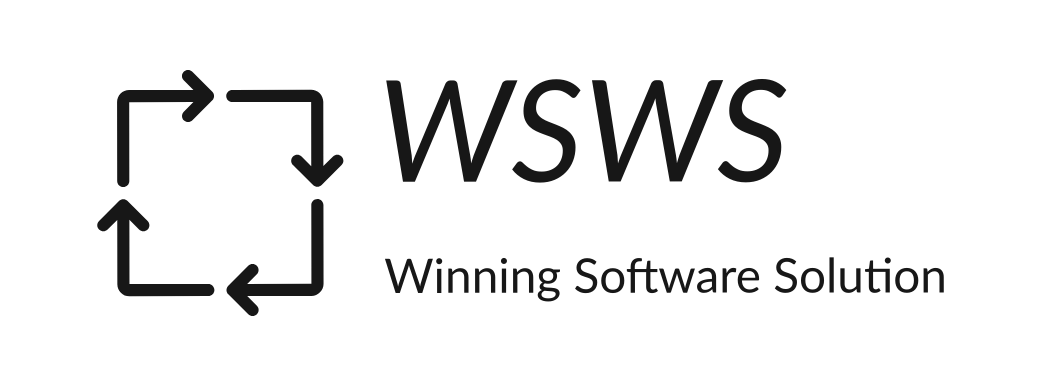
\includegraphics[width=0.4\textwidth]{../../template/WSWS-logos_transparent_crop}\\

		{\Large Winning Software Solution}\\[6pt]
		\href{mailto://winningsoftwaresolution@gmail.com}{winningsoftwaresolution@gmail.com}\\
		
		\ifdefined\progetto
		\vspace{1cm}
		{\Large\progetto}
		{\large\committenti}
		\else\fi
		
		\vspace{1.5cm}
		{\LARGE\titolo}
		
		\vfill
		
		\begin{tabular}{r | l}
		\multicolumn{2}{c}{\textit{Informazioni}}\\
		\hline
		
		\ifdefined\redattori
			\textit{Redattori} &
			\makecell[l]{\redattori}\\
		\else\fi
		\ifdefined\revisori
			\textit{Revisori} &
			\makecell[l]{\revisori}\\
		\else\fi
		\ifdefined\responsabili
			\textit{Respondabili} &
			\makecell[l]{\responsabili}\\
		\else\fi
		
		\ifdefined\versione
			\textit{Versione} & \versione
		\else\fi
		
		\textit{Uso} & \uso
		
		\end{tabular}
		
		\vspace{2cm}
		
		\ifdefined\descrizione
		Descrizione
		\vspace{6pt}
		\hrule
		\descrizione
		\else\fi
		\end{center}
	\end{titlepage}
}
\usepackage{hyperref}
\usepackage{array}
\usepackage{tabularx}

\def\vers#1-#2-#3-#4-#5\\{#1&#2&#3&#4&#5\\\hline}

\newcommand{\addversione}[5]{
	\ifdefined\versioni
		\let\old\versioni
		\renewcommand{\versioni}{#1&#2&#3&#4&#5\\\hline\old}
	\else
		\newcommand{\versioni}{#1&#2&#3&#4&#5\\\hline}
	\fi
}

\newcommand{\setversioni}[1]{\newcommand{\versioni}{#1}}

\newcommand{\makeversioni}{
	\begin{center}
		\begin{tabularx}{\textwidth}{|c|c|c|c|X|}
		\hline
		\textbf{Versione} & \textbf{Data} & \textbf{Persona} & \textbf{Attivtà} & \textbf{Descrizione} \\
		\hline
		\versioni
		\end{tabularx}
	\end{center}
	\clearpage
}

\settitolo{Analisi dei requisiti - v1.0.3} 
\setprogetto{ShopChain}
\setcommittenti{SyncLab}
\setredattori{Alberto Nicoletti\\Andrea Volpe}
\setrevisori{Giovanni Cocco}
\setresponsabili{Elia Scandaletti}
\setdestuso{esterno}
\setdescrizione{
Analisi dei requisiti del progetto ShopChain con casi d'uso e requisiti.
}

\addversione{0.0.0}{11/12/2021}{Alberto Nicoletti}{Redazione}{Strutturazione del documento}
\addversione{0.0.1}{03/01/2021}{Andrea Volpe}{Redazione}{Stesura casi d'uso}
\addversione{0.0.2}{21/01/2022}{Alberto Nicoletti}{Redazione}{Stesura requisiti}
\addversione{0.0.3}{21/01/2022}{Andrea Volpe}{Redazione}{Riorganizzazione requisiti}
\addversione{0.1.0}{04/02/2022}{Giovanni Cocco}{Revisione}{Correzioni varie}
\addversione{0.1.1}{05/02/2022}{Alberto Nicoletti}{Redazione}{Adeguamento casi d'uso a tecnologie scelte}
\addversione{0.1.2}{07/02/2022}{Andrea Volpe}{Redazione}{Modifica dei requisiti come concordato nell'incontro del 04/02/2022}
\addversione{1.0.0}{09/02/2022}{Elia Scandaletti}{Approvazione}{Approvazione per RTB}
\addversione{1.0.1}{01/03/2022}{Giovanni Cocco}{Redazione}{Approfondimento requisiti funzionali}
\addversione{1.0.2}{01/03/2022}{Elia Scandaletti}{Redazione}{Applicazione indicazioni del prof. Cardin}
\addversione{1.0.3}{11/03/2022}{Alberto Nicoletti}{Redazione}{Applicazione indicazioni del prof. Cardin}
\addversione{1.1.0}{01/04/2022}{Andrea Volpe}{Redazione}{Riadattato casi d'uso e requisiti in base alle nuove modifiche}


\begin{document}

\makefrontpage

\makeversioni

\tableofcontents
\pagebreak

\section{Introduzione}
\subsection{Scopo del documento}
Lo scopo del documento è raccogliere i risultati dell'attività di analisi dei requisiti. Contiene quindi la descrizione dei casi d'uso del prodotto software da sviluppare, ed i requisiti suddivisi per tipologia. Si vuole così dimostrare una completa comprensione del problema e delle aspettative della soluzione. I casi d'uso, ma soprattutto i requisiti saranno tenuti in considerazione nelle fasi di progettazione, di verifica e di validazione.
\subsection{Riferimenti}
\paragraph{Riferimenti normativi}
\begin{itemize}
    \item \underline{\href{https://www.math.unipd.it/~tullio/IS-1/2021/Progetto/C2.pdf}{Capitolato d'appalto C2}};
    \item \underline{\href{https://github.com/iota97/WinningSoftwareSolution/blob/main/public/interni/norme_di_progetto_v2.0.0.pdf}{Norme di Progetto}};
    \item \underline{\href{https://github.com/iota97/WinningSoftwareSolution/blob/main/public/esterni/verbali/2021_10_28_E.pdf}{Verbale esterno 2021/10/28}};
    \item \underline{\href{https://github.com/iota97/WinningSoftwareSolution/blob/main/public/esterni/verbali/2021_11_12_E.pdf}{Verbale esterno 2021/11/12}};
    \item \underline{\href{https://github.com/iota97/WinningSoftwareSolution/blob/main/public/esterni/verbali/2021_12_22_E.pdf}{Verbale esterno 2021/12/22}};
    \item \underline{\href{https://github.com/iota97/WinningSoftwareSolution/blob/main/public/interni/verbali/2021_12_23_I.pdf}{Verbale interno 2021/12/23}}.
\end{itemize}
\paragraph{Riferimenti informativi}
\begin{itemize}
    \item \underline{\href{https://www.math.unipd.it/~tullio/IS-1/2021/Dispense/T07.pdf}{Slide analisi dei requisiti - Materiale didattico del corso IS}};
    \item \underline{\href{https://www.math.unipd.it/~rcardin/swea/2022/Diagrammi\%20Use\%20Case.pdf}{Slide diagrammi dei casi d'uso - Materiale didattico del corso IS}}.
\end{itemize}

\section{Descrizione del prodotto}
L'azienda \textit{SyncLab} propone, attraverso il capitolato C2: \textit{ShopChain - Exchange Platform on
BlockChain}. L'obiettivo è sviluppare un sistema di pagamento sicuro e \textit{super partes} per E-commerce che trattenga i fondi durante la spedizione e che li sblocchi all'arrivo del pacco. Ciò consiste nella realizzazione su blockchain di un contratto digitale che si incarichi di ricevere l’ammontare in criptovaluta, lo trattenga, e lo consegni al venditore solo quando il pacco viene recapitato all’acquirente.
\subsection{Scopo del prodotto}
Il progetto consiste nello sviluppo di una piattaforma su blockchain con lo scopo di rendere automatizzato e sicuro lo smistamento dei fondi da clienti a E-commerce. Il processo di trasferimento del denaro avviene seguendo queste fasi:
\begin{enumerate}
\item caricamento dei dati dell'ordine di acquisto su contratto digitale;
\item trasferimento del denaro dal wallet dell'acquirente al contratto;
\item notifica al venditore dell'avvenuto pagamento;
\item conferma di ricezione del pacco da parte dell'acquirente tramite scannerizzazione di un QR Code sul pacco del prodotto acquistato;
\item invio del denaro dal contratto al wallet del venditore.
\end{enumerate}
\subsection{Parti del prodotto}
Il prodotto software è composto dalle seguenti parti:
\begin{itemize}
\item smart contract nella blockchain per la gestione di tutte le fasi del processo di trasferimento del denaro;
\item script per la messa in vendita automatizzata su contratto da integrare nel backend del venditore;
\item landing page per il pagamento da parte dell'acquirente;
\item piattaforma web per la visualizzazione e gestione delle transazioni da parte di sia venditore sia acquirente;
\item webapp che consente lo sblocco dei fondi dal contratto.
\end{itemize}
\subsection{Caratteristiche utenti}
Gli utenti di \textit{ShopChain} possono essere suddivisi in due categorie:
\begin{itemize}
\item venditore: gli amministratori di un sito di e-commerce che vogliono aggiungere \textit{ShopChain} come metodo di pagamento;
\item acquirente: I clienti di un sito di e-commerce che scelgono di utilizzare \textit{ShopChain} come metodo di pagamento per i prodotti da acquistare.
\end{itemize}
Tutti gli utenti devono essere in possesso di un wallet compatibile con la blockchain scelta per questo Progetto.
Non potendo prevedere con accuratezza quanti e quali e-commerce decideranno di utilizzare \textit{ShopChain} altre considerazioni sulle caratteristiche di utenza sono superflue. Il prodotto deve essere facilmente integrabile in quante più tipologie di e-commerce possibili.

\subsection{Vincoli e preferenze}
Il proponente non impone vincoli nella scelta delle tecnologie, ma ci sono comunque dei suggerimenti da considerare:
\begin{itemize}
\item utilizzo di blockchain pubblica;
\item utilizzo di Java e Angular per lo sviluppo delle parti di Back-end e di Front-end della componente web application del sistema;
\item utilizzo di database PostgreSQL.
\end{itemize}

Per il completamento del progetto il proponente richiede che siano ottenuti i seguenti risultati:
\begin{itemize}
\item server, completo di UI;
\item test che dimostrino il corretto funzionamento dei servizi e delle funzionalità previste, con una copertura minima dell'80\% correlata di report;
\item documentazione su scelte implementative e progettuali effettuate, le relative motivazioni, i problemi aperti e le eventuali soluzioni proposte da esplorare.
\end{itemize}

\section{Casi d'uso}
\subsection{Attori}
\begin{itemize}
\item \textbf{Venditore con wallet connesso}: venditore che ha già connesso il proprio wallet con Metamask;
\item \textbf{venditore con wallet non connesso}: venditore che non ha ancora connesso il proprio wallet con Metamask;
\item \textbf{acquirente con wallet connesso}: acquirente che ha già connesso il proprio wallet con Metamask;
\item \textbf{acquirente con wallet non connesso}: acquirente che non ha ancora connesso il proprio wallet con Metamask;
\item \textbf{e-commerce}: backend dell'e-commerce;
\item \textbf{metamask}: applicativo di terze parti per la gestione dei wallet;
\item \textbf{database}: persistenze SQL interna al nostro sistema.
\end{itemize}

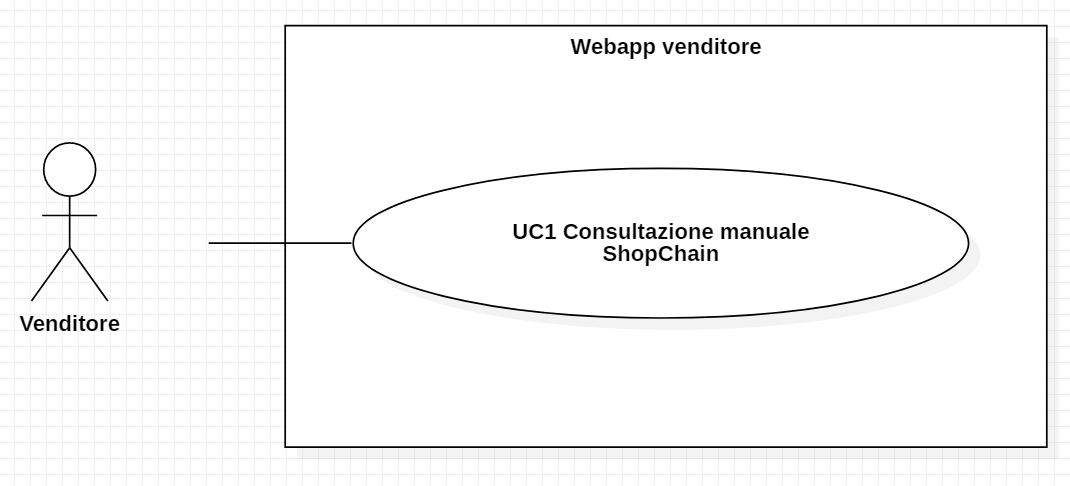
\includegraphics[width=0.7\textwidth]{UC_WAV1}
\captionof{figure}{Caso d'uso UC1}

\paragraph{UC1 - Consultazione manuale ShopChain}\\
\textbf{Attori primari}: Venditore con wallet connesso.\\
\textbf{Precondizioni}: Il venditore usa il servizio ShopChain e vorrebbe avere più informazioni sul suo utilizzo.\\
\textbf{Postcondizioni}: Il venditore consulta il manuale utente di ShopChain.\\
\textbf{Scenario principale}:
\begin{enumerate}
\item Al venditore viene fornito il manuale utente già dall'acquisizione del prodotto ShopChain.
\item Il venditore è libero di consultare il manuale in ogni momento.
\end{enumerate}
\textbf{Requisiti collegati}: RVO03.

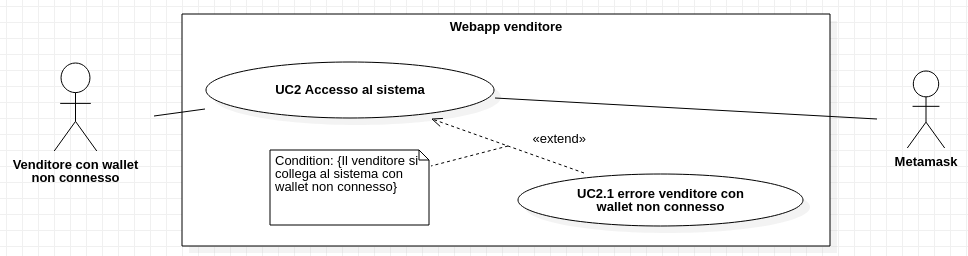
\includegraphics[width=0.9\textwidth]{UC_WAV2}
\captionof{figure}{Caso d'uso UC2}

\paragraph{UC2 - Accesso al sistema (webapp venditore)}\\
\textbf{Attore primario}: Venditore con wallet non connesso.\\
\textbf{Attore secondario}: Metamask.\\
\textbf{Precondizioni}: Il venditore vuole accedere alla webapp.\\
\textbf{Postcondizioni}: Il venditore si è connesso alla webapp con Metamask.\\
\textbf{Scenario principale}:
Il venditore usando Metamask, si connette alla webapp con il proprio wallet.\\
\textbf{Requisiti collegati}: RFO01, RFO34.
\textbf{Estensione}:
UC2.1 Errore venditore con wallet non connesso:
\begin{enumerate}
    \item Il sistema mostra un messaggio di errore wallet non connesso.
    \item Il sistema non permette al venditore di entrare nel sistema.
\end{enumerate}
\textbf{Requisiti collegati all'estensione UC2.1}: RFO02.

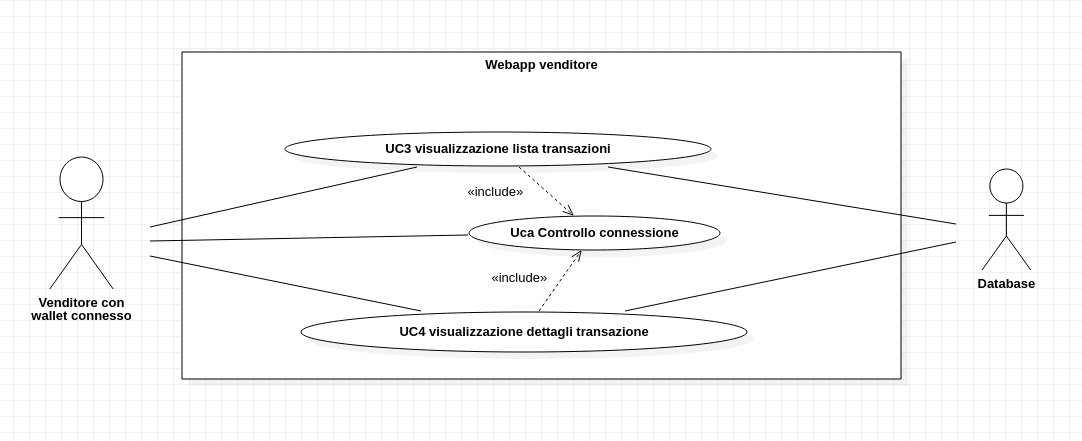
\includegraphics[width=0.9\textwidth]{UC_WAV3}
\captionof{figure}{Casi d'uso UC3 e UC4}

\paragraph{UC3 - visualizzazione lista transazioni}\\
\textbf{Attore primario}: Venditore con wallet connesso. \\
\textbf{Attore secondario}: Database. \\
\textbf{Precondizioni}: Il venditore ha effettuato l'accesso al sistema.\\
\textbf{Postcondizioni}:  Il venditore vede la lista delle transazioni.\\
\textbf{Scenario principale}:
\begin{enumerate}
\item Il venditore vede la lista delle transazioni;
\item Il venditore può scegliere che tipo di transazioni vedere (tutte, completate, in attesa);
\item Il sistema mostra al venditore l'elenco delle transazioni richieste.
\end{enumerate}
\textbf{Requisiti collegati}: RFO03, RFO35, RFO36.

\paragraph{UC4 - visualizzazione dettaglio transazione}\\
\textbf{Attore primario}: Venditore con wallet connesso.\\
\textbf{Attore secondario}: Database\\
\textbf{Precondizioni}: Il venditore ha acceduto alla funzionalità di visualizzazione della lista delle transazioni.\\
\textbf{Postcondizioni}: Il venditore vede i dettagli di una singola transazione.\\
\textbf{Scenario principale}:
\begin{enumerate}
\item Il venditore seleziona una delle transazioni dall'elenco;
\item Il venditore visualizza i dettagli della singola transazione.
\end{enumerate}
\textbf{Requisiti collegati}: RFO37, RFO38, RFO40.

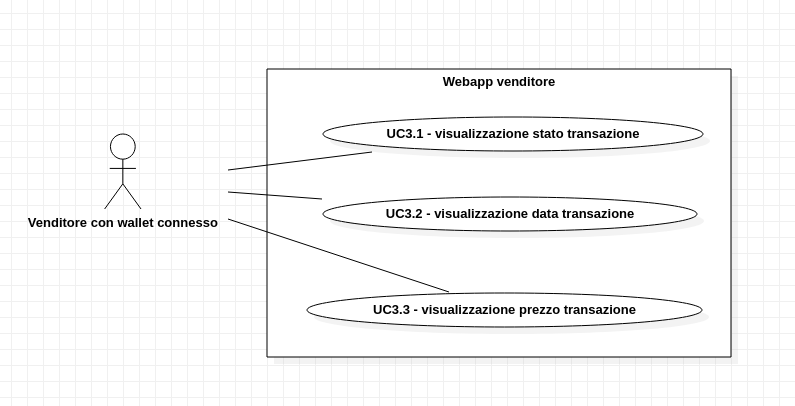
\includegraphics[width=0.9\textwidth]{UC3D}
\captionof{figure}{Casi d'uso UC3.1, UC3.2 ed UC3.3}

\paragraph{UC3.1 - Visualizzazione stato transazioni}\\
\textbf{Attore primario}: Venditore con wallet connesso.\\
\textbf{Precondizioni}: Il venditore vuole visualizzare lo stato delle transazioni.\\
\textbf{Postcondizioni}: Il venditore visualizza lo stato delle transazioni.\\
\textbf{Scenario principale}: Viene visualizzato lo stato delle transazioni.\\

\paragraph{UC3.2 - Visualizzazione data transazioni}\\
\textbf{Attore primario}: Venditore con wallet connesso.\\
\textbf{Precondizioni}: Il venditore vuole visualizzare la data delle transazioni.\\
\textbf{Postcondizioni}: Il venditore visualizza la data delle transazioni.\\
\textbf{Scenario principale}: Viene visualizzato la data delle transazioni.\\

\paragraph{UC3.3 - Visualizzazione prezzo transazioni}\\
\textbf{Attore primario}: Venditore con wallet connesso.\\
\textbf{Precondizioni}: Il venditore vuole visualizzare il prezzo delle transazioni.\\
\textbf{Postcondizioni}: Il venditore visualizza il prezzo delle transazioni.\\
\textbf{Scenario principale}: Viene visualizzato il prezzo delle transazioni.\\



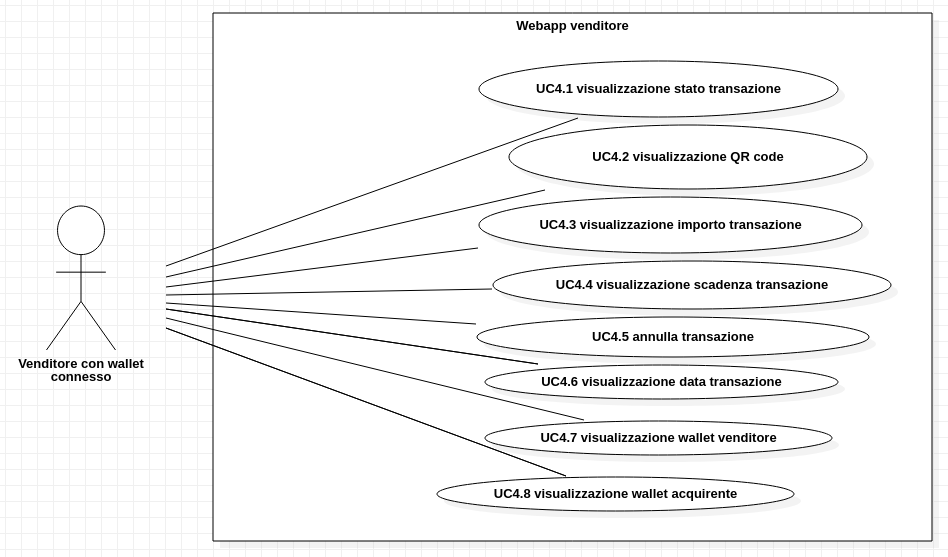
\includegraphics[width=0.9\textwidth]{UC_WAV4}
\captionof{figure}{Casi d'uso UC4.1, UC4.2, UC4.3, UC4.4, UC4.5, UC4.6, UC4.7, UC4.8}

\paragraph{UC4.1 - Visualizzazione stato transazione}\\
\textbf{Attore primario}: Venditore con wallet connesso.\\
\textbf{Precondizioni}: Il venditore vuole visualizzare lo stato di una transazione.\\
\textbf{Postcondizioni}: Il venditore visualizza lo stato di una transazione.\\
\textbf{Scenario principale}: Viene visualizzato lo stato della transazione.\\
\textbf{Requisiti collegati}: RFO04.

\paragraph{UC4.2 - Visualizzazione QR Code}\\
\textbf{Attore primario}: Venditore con wallet connesso.\\
\textbf{Precondizioni}: Il venditore vuole ottenere il QR Code di una transazione in attesa.\\
\textbf{Postcondizioni}: Il venditore è in possesso del QR Code da applicare sul pacco del prodotto.\\
\textbf{Scenario principale}:
\begin{enumerate}
\item Viene visualizzato il QR Code della transazione in attesa selezionata;
\item Il venditore può stampare il QR Code applicarlo sul pacco del prodotto.
\end{enumerate}
\textbf{Requisiti collegati}: RFO05, RFO51.

\paragraph{UC4.3 - Visualizzazione importo transazione}\\
\textbf{Attore primario}: Venditore con wallet connesso.\\
\textbf{Precondizioni}: Il venditore vuole visualizzare l'importo di una transazione.\\
\textbf{Postcondizioni}: Il venditore visualizza l'importo di una transazione.\\
\textbf{Scenario principale}: Viene visualizzato l'importo della transazione in dollari.\\
\textbf{Requisiti collegati}: RFO06.

\paragraph{UC4.4 - Visualizzazione scadenza transazione}\\
\textbf{Attore primario}: Venditore  con wallet connesso.\\
\textbf{Precondizioni}: Il venditore vuole visualizzare la scadenza di una transazione.\\
\textbf{Postcondizioni}: Il venditore visualizza la scadenza di una transazione.\\
\textbf{Scenario principale}: Il venditore vede la data della scadenza di una transazione, oltre la quale l'acquirente riceverà indietro la valuta bloccata.\\
\textbf{Requisiti collegati}: RFO07, RFO39, RFO41.

\paragraph{UC4.5 - annulla transazione}\\
\textbf{Attore primario}: Venditore  con wallet connesso.\\
\textbf{Precondizioni}: Il venditore vuole annullare una transazione in attesa.\\
\textbf{Postcondizioni}: La transazione è stata annullata ed i fondi sono stati restituiti all'acquirente.\\
\textbf{Scenario principale}: Il venditore annulla una transizione in stato di attessa ed i fondi vengono restituiti all'acquirente.\\
\textbf{Requisiti collegati}: RFO51.

\paragraph{UC4.6 - visualizzazione data transazione}\\
\textbf{Attore primario}: Venditore con wallet connesso.\\
\textbf{Precondizioni}: Il venditore vuole visualizzare la data di creazione una transazione.\\
\textbf{Postcondizioni}: Il venditore visualizza la data di creazione di una transazione.\\
\textbf{Scenario principale}: Il venditore vede la data di creazione di una transazione.\\
\textbf{Requisiti collegati}: RFOX.

\paragraph{UC4.7 - visualizzazione wallet venditore}\\
\textbf{Attore primario}: Venditore con wallet connesso.\\
\textbf{Precondizioni}: Il venditore vuole visualizzare il wallet del venditore.\\
\textbf{Postcondizioni}: Il venditore vuole visualizzare il wallet del venditore.\\
\textbf{Scenario principale}: Il venditore visualizza il wallet del venditore.\\
\textbf{Requisiti collegati}: RFOX.

\paragraph{UC4.8 - visualizzazione wallet acquirente}\\
\textbf{Attore primario}: Venditore con wallet connesso.\\
\textbf{Precondizioni}: Il venditore vuole visualizzare il wallet dell'acquirente.\\
\textbf{Postcondizioni}: Il venditore vuole visualizzare il wallet dell'acquirente.\\
\textbf{Scenario principale}: Il venditore visualizza il wallet dell'acquirente.\\
\textbf{Requisiti collegati}: RFOX.

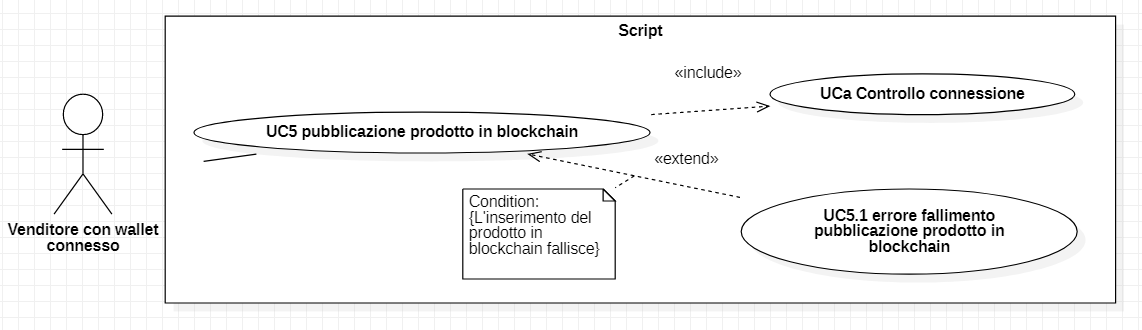
\includegraphics[width=0.9\textwidth]{UC_script}
\captionof{figure}{Casi d'uso UC5 e UC5.1}


\paragraph{UC5 - Pubblicazione prodotto in blockchain}\\
\textbf{Attore primario}: E-commerce.\\
\textbf{Precondizioni}: L'e-commerce ha integrato lo script nel proprio backend.\\
\textbf{Postcondizioni}: Lo script nell'e-commerce ha pubblicato il nuovo prodotto in blockchain.\\
\textbf{Scenario principale}:
\begin{enumerate}
    \item Il venditore inserisce un nuovo prodotto nell'e-commerce;
    \item Tramite lo script il prodotto viene pubblicato in blockchain;
    \item Il prodotto è pubblico in blockchain e utilizzabile per fare nuove transazioni.
\end{enumerate}
\textbf{Requisiti collegati}: RFO09, RFO43, RFD44, RVO06.\\
\textbf{Estensione}:
\begin{enumerate}
    \item UC5.1 Errore fallimento pubblicazione prodotto in blockchain:\\
\end{enumerate}
lo script salva in un file di log il messaggio di errore.\\
\textbf{Requisiti collegati all'estensione UC5.1}: RFO10.

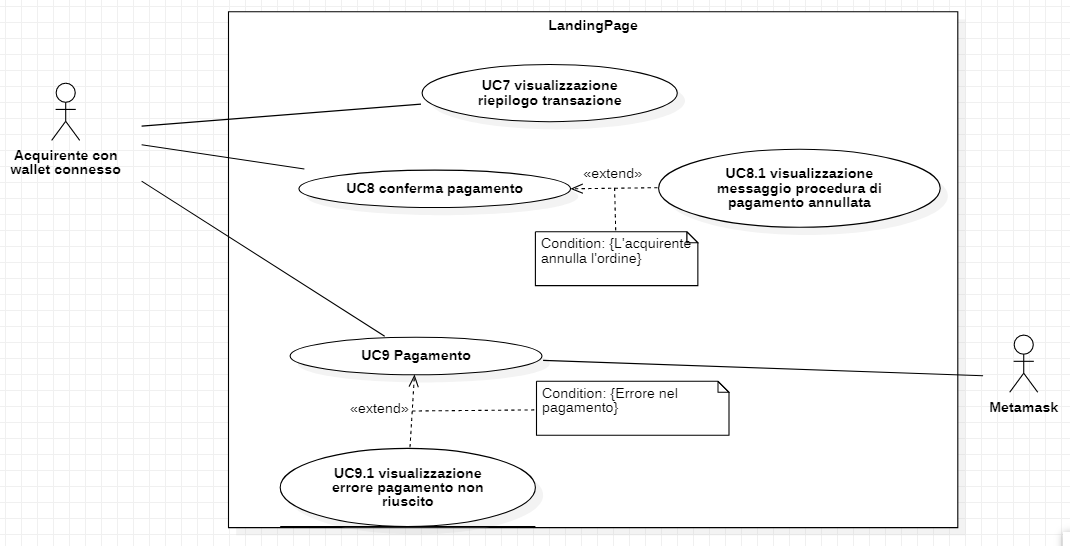
\includegraphics[width=0.9\textwidth]{UC_LP2}
\captionof{figure}{Casi d'uso UC7, UC8, UC8.1, UC9 e UC9.1}

\paragraph{UC7 - Visualizzazione riepilogo transazione}\\
\textbf{Attore primario}: Acquirente con wallet connesso.\\
\textbf{Precondizioni}: L'acquirente con wallet connesso vuole effettuare un acquisto usando ShopChain.\\
\textbf{Postcondizioni}: Il sistema mostra il riepilogo della transazione.\\
\textbf{Scenario principale}:
Viene mostrato all'acquirente il riepilogo della transazione con il prezzo in dollari da pagare.\\
\textbf{Requisiti collegati}: RFO13.

\paragraph{UC8 - Conferma pagamento}\\
\textbf{Attore primario}: Acquirente con wallet connesso.\\
\textbf{Precondizioni}: L'acquirente sta effettuando un acquisto e il sistema mostra il riepilogo della transazione.\\
\textbf{Postcondizioni}: L'acquirente ha confermato il pagamento.\\
\textbf{Scenario principale}:
\begin{enumerate}
    \item Il sistema mostra il riepilogo della transazione;
    \item L'acquirente conferma l'ordine.
\end{enumerate}
\textbf{Requisiti collegati}: RFO14.\\
\textbf{Estensione}:
UC8.1 Reindirizzamento acquirente in e-commerce:
\begin{enumerate}
    \item L'acquirente annulla il pagamento dalla landing page;
    \item Il pagamento non viene completato con successo;
    \item L'acquirente viene reindirizzato al sito web dell'e-commerce.
\end{enumerate}
\textbf{Requisiti collegati all'estensione UC8.1}: RFO15, RFO16.

\paragraph{UC9 - Pagamento}\\
\textbf{Attore primario}: Acquirente con wallet connesso.\\
\textbf{Attore secondario}: Metamask.\\
\textbf{Precondizioni}: L'acquirente ha confermato il pagamento.\\
\textbf{Postcondizioni}: Il pagamento è stato completato con successo.\\
\textbf{Scenario principale}:
\begin{enumerate}
    \item L'acquirente avvia la procedura di pagamento;
    \item L'acquirente effettua il pagamento tramite Metamask;
    \item L'ordine è stato pagato.
\end{enumerate}
\textbf{Requisiti collegati}: RFO17, RFO47.\\
\textbf{Estensione}:
UC9.1 Annullamento pagamento:
\begin{enumerate}
    \item Il pagamento tramite Metamask fallisce;
    \item Il pagamento non viene completato con successo;
    \item L'acquirente può nuovamente confermare il pagamento (UC8);
\end{enumerate}
\textbf{Requisiti collegati all'estensione UC9.1}: RFO18.

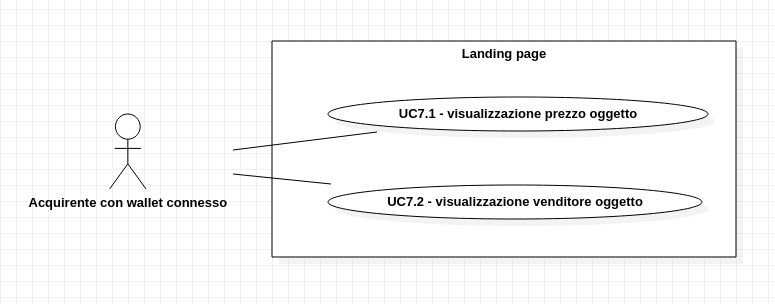
\includegraphics[width=0.9\textwidth]{UC7D}
\captionof{figure}{Casi d'uso UC7.1 e UC7.2}

\paragraph{UC7.1 - Visualizzazione prezzo oggetto}\\
\textbf{Attore primario}: Acquirente con wallet connesso.\\
\textbf{Precondizioni}: L'Acquirente vuole visualizzare il prezzo dell'oggetto.\\
\textbf{Postcondizioni}: L'Acquirente visualizza il prezzo dell'oggetto.\\
\textbf{Scenario principale}: Viene visualizzato il prezzo dell'oggetto.\\

\paragraph{UC7.2 - Visualizzazione il venditore dell'oggetto}\\
\textbf{Attore primario}: Acquirente con wallet connesso.\\
\textbf{Precondizioni}: L'Acquirente vuole visualizzare il venditore dell'oggetto.\\
\textbf{Postcondizioni}: L'Acquirente visualizza il venditore dell'oggetto.\\
\textbf{Scenario principale}: Viene visualizzato il venditore dell'oggetto.\\

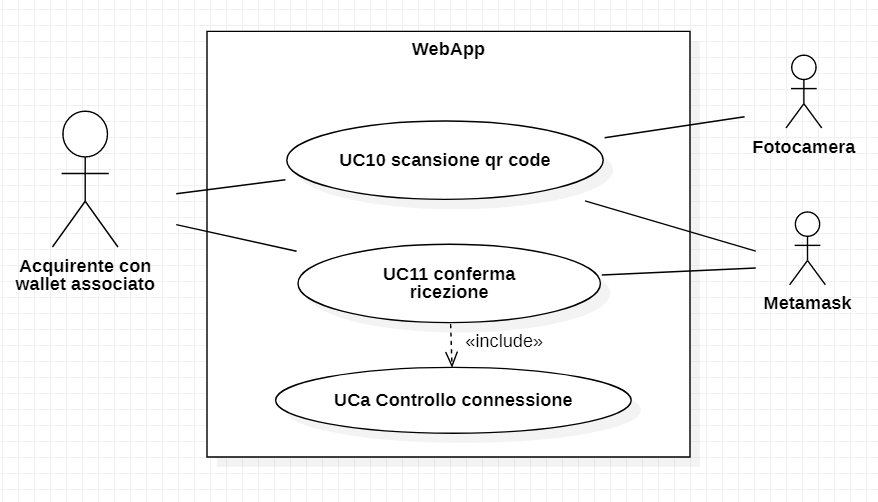
\includegraphics[width=0.9\textwidth]{UC_WAA1}
\captionof{figure}{Caso d'uso UC10}


\paragraph{UC10 - Accesso al sistema (WebApp Acquirente)}\\
\textbf{Attore primario}: Acquirente con wallet non connesso.\\
\textbf{Attore secondario}: Metamask.\\
\textbf{Precondizioni}: L'acquirente nella webapp acquirente non è connesso con Metamask.\\
\textbf{Postcondizioni}: L'acquirente accede al sistema.\\
\textbf{Scenario principale}:
L'acquirente usando Metamask, si connette con il proprio wallet.
\textbf{Requisiti collegati}: RFO19.

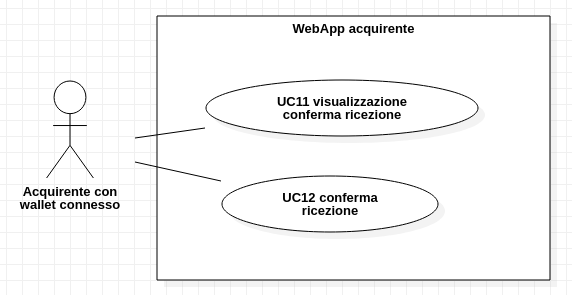
\includegraphics[width=0.9\textwidth]{UC_WAA2}
\captionof{figure}{Casi d'uso UC11, UC12}

\paragraph{UC11 - Visualizzazione conferma ricezione}\\
\textbf{Attore primario}: Acquirente con wallet connesso.\\
\textbf{Precondizioni}: L'acquirente è connesso con Metamask ed è arrivato alla pagina di conferma ricezione scansionando il QR Code sul pacco del prodotto.\\
\textbf{Postcondizioni}: L'acquirente visualizza la pagina della transazione relativa al pacco appena ricevuto.\\
\textbf{Scenario principale}:
Vengono mostrati i dati relativi alla transazione e un pulsante per confermare la ricezione del pacco.\\
\textbf{Requisiti collegati}: RFO21.

\paragraph{UC12 - Conferma ricezione}\\
\textbf{Attore primario}: Acquirente con wallet connesso.\\
\textbf{Precondizioni}: L'acquirente è connesso con Metamask alla pagina di conferma ricezione e conferma la ricezione del pacco.\\
\textbf{Postcondizioni}: L'acquirente ha confermato la ricezione del pacco, i fondi sono stati sbloccati.\\
\textbf{Scenario principale}:
\begin{enumerate}
    \item L'acquirente controlla sia tutto corretto e conferma la ricezione del pacco;
    \item Il denaro viene sbloccato e mandato nel wallet del venditore.
\end{enumerate}
\textbf{Requisiti collegati}: RFO22, RFO45, RFO46.\\

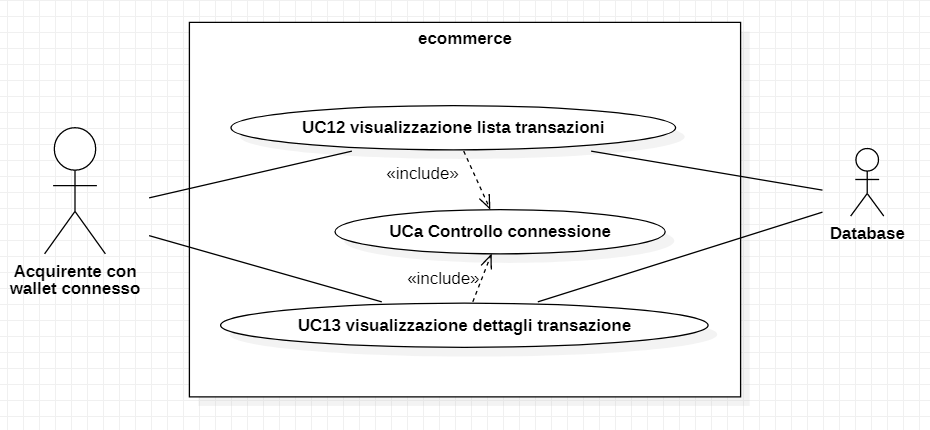
\includegraphics[width=0.9\textwidth]{UC_ECA1}
\captionof{figure}{Caso d'uso UC13}

\paragraph{UC13 - Accesso al sistema (pagina lista transazioni acquirente in e-commerce)}\\
\textbf{Attore primario}: Acquirente con wallet non connesso.\\
\textbf{Attore secondario}: Metamask.\\
\textbf{Precondizioni}: L'acquirente, nella pagina con la sua lista delle transazioni in e-commerce, non è connesso con Metamask.\\
\textbf{Postcondizioni}: L'acquirente accede alla pagina con la sua lista delle transazioni in e-commerce.\\
\textbf{Scenario principale}:
L'acquirente usando Metamask, si connette con il proprio wallet.\\
\textbf{Requisiti collegati}: RFO24, RFO48.

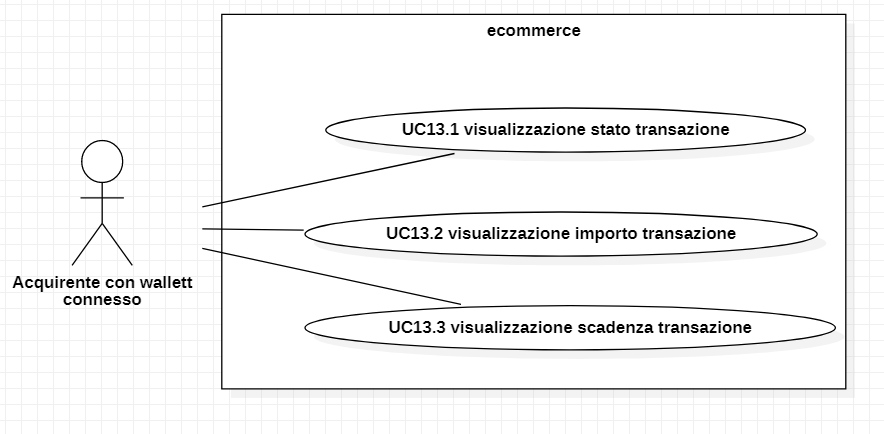
\includegraphics[width=0.9\textwidth]{UC_ECA2}
\captionof{figure}{Casi d'uso UC14 e UC15}

\paragraph{UC14 visualizzazione lista transazioni}\\
\textbf{Attore primario}: Acquirente con wallet connesso. \\
\textbf{Attore secondario}: Database. \\
\textbf{Precondizioni}: L'acquirente ha effettuato l'accesso al sistema.\\
\textbf{Postcondizioni}:  L'acquirente vede la lista delle transazioni.\\
\textbf{Scenario principale}:
\begin{enumerate}
\item L'acquirente vede la lista delle transazioni;
\item L'acquirente può scegliere che tipo di transazioni vedere (tutte, completate, in attesa);
\item Il sistema mostra all'acquirente l'elenco delle transazioni richieste.
\end{enumerate}
\textbf{Requisiti collegati}: RFO26, RFO49.

\paragraph{UC15 - visualizzazione dettaglio transazione}\\
\textbf{Attore primario}: Acquirente con wallet connesso.\\
\textbf{Attore secondario}: Database.\\
\textbf{Precondizioni}: L'acquirente ha acceduto alla funzionalità di visualizzazione della lista delle transazioni.\\
\textbf{Postcondizioni}: L'acquirente vede i dettagli di una singola transazione.\\
\textbf{Scenario principale}:
\begin{enumerate}
\item L'acquirente seleziona una delle transazioni dall'elenco;
\item L'acquirente visualizza i dettagli della singola transazione.
\end{enumerate}
\textbf{Requisiti collegati}: RFO11, .

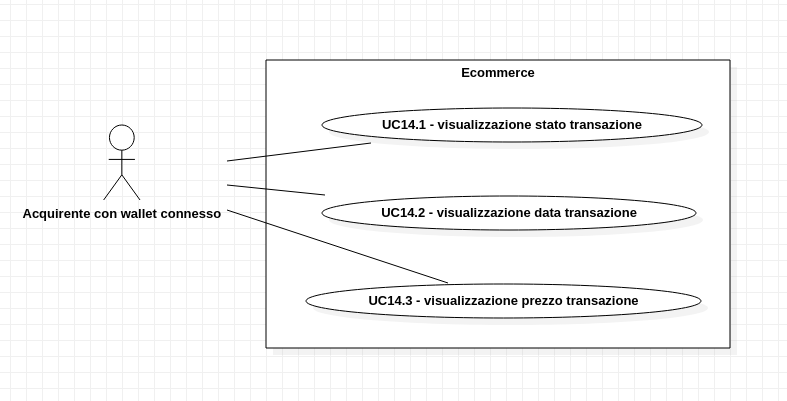
\includegraphics[width=0.9\textwidth]{UC14D}
\captionof{figure}{Casi d'uso UC14.1, UC14.2 e UC14.3}

\paragraph{UC14.1 - Visualizzazione stato transazioni}\\
\textbf{Attore primario}: Acquirente con wallet connesso.\\
\textbf{Precondizioni}: L'Acquirente vuole visualizzare lo stato delle transazioni.\\
\textbf{Postcondizioni}: L'Acquirente visualizza lo stato delle transazioni.\\
\textbf{Scenario principale}: Viene visualizzato lo stato delle transazioni.\\

\paragraph{UC14.2 - Visualizzazione data transazioni}\\
\textbf{Attore primario}: Acquirente con wallet connesso.\\
\textbf{Precondizioni}: L'Acquirente vuole visualizzare la data delle transazioni.\\
\textbf{Postcondizioni}: L'Acquirente visualizza la data delle transazioni.\\
\textbf{Scenario principale}: Viene visualizzato la data delle transazioni.\\

\paragraph{UC14.3 - Visualizzazione prezzo transazioni}\\
\textbf{Attore primario}: Acquirente con wallet connesso.\\
\textbf{Precondizioni}: L'Acquirente vuole visualizzare il prezzo delle transazioni.\\
\textbf{Postcondizioni}: L'Acquirente visualizza il prezzo delle transazioni.\\
\textbf{Scenario principale}: Viene visualizzato il prezzo delle transazioni.\\


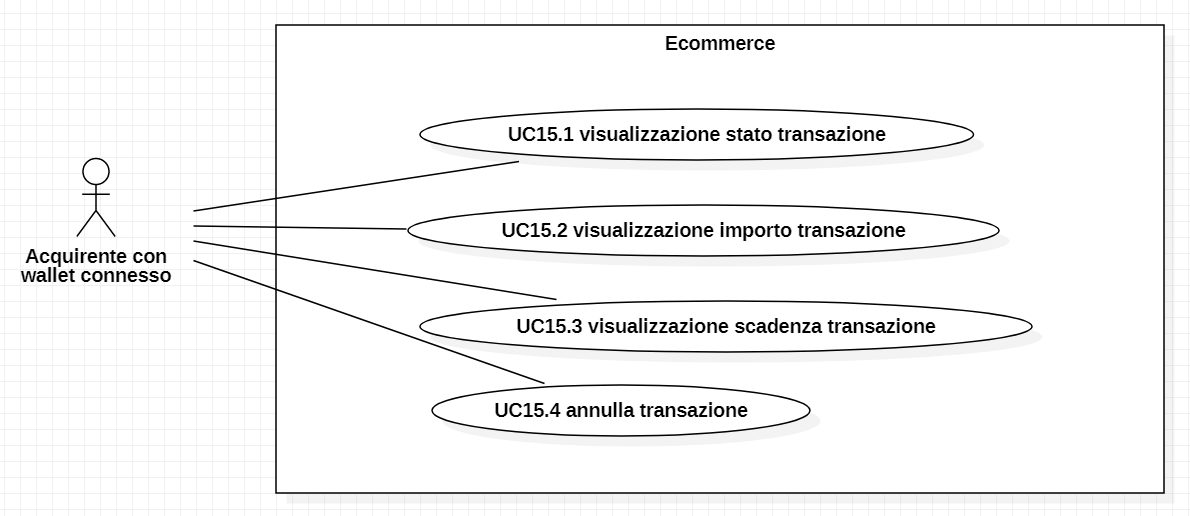
\includegraphics[width=0.9\textwidth]{UC_ECA3}
\captionof{figure}{Casi d'uso UC15.1, UC15.2, UC15.3, UC15.4, UC15.5, UC15.6 ed UC15.7}

\paragraph{UC15.1 - Visualizzazione stato transazione}\\
\textbf{Attore primario}: Acquirente con wallet connesso.\\
\textbf{Precondizioni}: L'acquirente vuole visualizzare lo stato di una transazione.\\
\textbf{Postcondizioni}: L'acquirente visualizza lo stato di una transazione.\\
\textbf{Scenario principale}: Viene mostrato lo stato della transazione: in attesa o completata.\\
\textbf{Requisiti collegati}: RFO27.

\paragraph{UC15.2 - Visualizzazione importo transazione}\\
\textbf{Attore primario}: Acquirente con wallet connesso.\\
\textbf{Precondizioni}: L'acquirente vuole visualizzare l'importo di una transazione.\\
\textbf{Postcondizioni}: L'acquirente visualizza l'importo di una transazione.\\
\textbf{Scenario principale}: Viene mostrato l'importo della transazione in dollari.\\
\textbf{Requisiti collegati}: RFO28, RFO29.

\paragraph{UC15.3 - Visualizzazione scadenza transazione}\\
\textbf{Attore primario}: Acquirente  con wallet connesso.\\
\textbf{Precondizioni}: L'acquirente vuole visualizzare la scadenza di una transazione in attesa.\\
\textbf{Postcondizioni}: L'acquirente visualizza la scadenza di una transazione in attesa.\\
\textbf{Scenario principale}: Viene visualizzata la data della scadenza di una transazione in attesa, oltre la quale l'acquirente riceverà indietro la valuta bloccata.\\
\textbf{Requisiti collegati}: RFO30.

\paragraph{UC15.4 - Annulla transazione}\\
\textbf{Attore primario}: Acquirente  con wallet connesso.\\
\textbf{Precondizioni}: L'acquirente vuole annullare una transazione in attesa dopo i 14 giorni.\\
\textbf{Postcondizioni}: La transazione è stata annullata e l'acquirente ha ricevuto i propri fondi.\\
\textbf{Scenario principale}: Il pacco non è arrivato entro i 14 giorni. Quindi l'acquirente può annullare la transazione.\\
\textbf{Requisiti collegati}: RFO52.

\paragraph{UC15.5 - Visualizzazione indirizzo wallet venditore}\\
\textbf{Attore primario}: Acquirente  con wallet connesso.\\
\textbf{Precondizioni}: L'acquirente vuole visualizzare l'indirizzo del wallet del venditore.\\
\textbf{Postcondizioni}: L'acquirente l'indirizzo del wallet del venditore.\\
\textbf{Scenario principale}: Viene mostrato l'indirizzo del wallet del venditore.\\
\textbf{Requisiti collegati}: RFO53.

\paragraph{UC15.6 - Visualizzazione indirizzo wallet acquirente}\\
\textbf{Attore primario}: Acquirente  con wallet connesso.\\
\textbf{Precondizioni}: L'acquirente vuole visualizzare l'indirizzo del wallet dell'acquirente.\\
\textbf{Postcondizioni}: L'acquirente l'indirizzo del wallet dell'acquirente.\\
\textbf{Scenario principale}: Viene mostrato l'indirizzo del wallet dell'acquirente.\\
\textbf{Requisiti collegati}: RFO54.

\paragraph{UC15.7 - Visualizzazione data transazione}\\
\textbf{Attore primario}: Acquirente  con wallet connesso.\\
\textbf{Precondizioni}: L'acquirente vuole visualizzare la data della transazione.\\
\textbf{Postcondizioni}: L'acquirente visualizza la data della transazione.\\
\textbf{Scenario principale}: Viene visualizzata la data della transazione.\\
\textbf{Requisiti collegati}: RFO55.

\section{Requisiti}
Ogni requisito è identificato da un codice univoco composto da: R(per requisito)+F/Q/V(per la tipologia: funzionale, qualità, vincolo)+O/D/F(per la rilevanza: obbligatorio, desiderabile, facoltativo)+x(un numero univoco a due cifre).
\subsection{Requisiti funzionali}

 \setlength\tabcolsep{4pt}
\begin{longtable}{|c|p{7cm}|c|p{4cm}|}
\hline
 \multicolumn{4}{| c |}{Requisiti funzionali}\\
 \hline
 Codice & Descrizione & Rilevanza & Fonti\\
 \hline
 \endfirsthead

 \hline
 \multicolumn{4}{| c |}{Requisiti funzionali}\\
 \hline
 Codice & Descrizione & Rilevanza & Fonti\\
 \hline
 \endhead
% WEBAPP VENDITORE
\hline
RFO01 & Per accedere alla webapp venditore il venditore con wallet non connesso deve connettere il proprio wallet tramite Metamask. & Obbligatorio & UC2 \\
\hline
RFO02 & Un venditore con wallet non connesso non può accedere alla webapp venditore. & Obbligatorio & UC2.1, \underline{\href{https://www.math.unipd.it/~tullio/IS-1/2021/Progetto/C2.pdf}{Capitolato}} \\
\hline
RFO34 & La webapp deve comunicare il wallet del venditore al server. & Obbligatorio & UC2\\
\hline
RFO03 & Il venditore deve poter visualizzare la lista delle transazioni nella webapp venditore. & Obbligatorio & UC3 \\
\hline
RFO35 & Il server deve fornire una pagina con la lista delle transazioni. & Obbligatorio & UC3 \\
\hline
RFO36 & La persistenza deve permettere di filtrare le transazioni per venditore. & Obbligatorio & UC3 \\
\hline
RFO04 & Il venditore deve poter visualizzare nella webapp venditore, per ogni transazione, il suo stato (attesa o completata). & Obbligatorio & UC4.1 \\
\hline
RFO05 & Il venditore deve poter visualizzare nella webapp venditore, per ogni transazione in attesa, il QR Code da applicare sul pacco. & Obbligatorio & UC4.2 \\
\hline
RFO51 & La webapp venditore deve poter generare data una stringa un QR Code. & Obbligatorio & UC4.2 \\
\hline
RFO06 & Il venditore deve poter visualizzare nella webapp venditore, per ogni transazione, l'importo in dollari. & Obbligatorio & UC4.3 \\
\hline
RFO07 & Il venditore deve poter visualizzare nella webapp venditore, per ogni transazione, la scadenza della transazione. & Obbligatorio & UC4.4 \\
\hline
RFOX & Il venditore deve poter visualizzare nella webapp venditore, per ogni transazione, la data di creazione della transazione. & Obbligatorio & UC4.6 \\
\hline
RFOX & Il venditore deve poter visualizzare nella webapp venditore, per ogni transazione, il wallet del venditore. & Obbligatorio & UC4.7 \\
\hline
RFOX & Il venditore deve poter visualizzare nella webapp venditore, per ogni transazione, il wallet dell'acquirente. & Obbligatorio & UC4.8 \\
\hline
RFO37 & Il server deve fornire una pagina con i dettagli di un transazione (prezzo, stato, data di creazione, data di chiusura, acquirente e venditore). & Obbligatorio & UC4 \\
\hline
RFO38 & La persistenza deve tener traccia dei dettagli di un transazione (prezzo, stato, data di creazione, data di chiusura, acquirente e venditore). & Obbligatorio & UC4 \\
\hline
RFO39 & La persistenza deve poter associare ad ogni transazione il proprio timestamp. & Obbligatorio & UC4.4 \\
\hline
RFO40 & La persistenza deve poter fornire i dati di una particolare transazione su richiesta del server. & Obbligatorio & UC4 \\
\hline
RFO41 & Lo smart contract deve rimborsare la valuta al compratore se sono passati 14gg dall'apertura della transazione & Obbligatorio & \underline{\href{https://github.com/iota97/WinningSoftwareSolution/blob/main/public/interni/verbali/2021_11_12_I.pdf}{Verbale del 12/11/2021}}, UC4.4 \\
\hline
% SCRIPT
RFO09 & Il prodotto deve essere pubblicato automaticamente in blockchain, quando il venditore inserisce un nuovo prodotto nell'e-commerce, grazie al nostro script incluso dal venditore nel suo e-commerce. & Obbligatorio & UC5 \\
\hline
RFO10 & Il nostro script deve salvare un messaggio di errore in un file di log, se la pubblicazione del prodotto in blockchain dall'e-commerce (grazie allo script) fallisce. & Obbligatorio & UC5.1 \\
\hline
RFO43 & Lo script deve ritornare l'id del prodotto inserito in blockchain. & Obbligatorio & UC5 \\
\hline
RFD44 & Lo script essere usabile sia come modulo python che come script python standalone. & Desiderabile & UC5 \\
\hline
% LANDING PAGE
RFO11 & Per accedere alla landing page l'acquirente con wallet non connesso deve connettere il proprio wallet tramite Metamask. & Obbligatorio & UC6, UC15 \\
\hline
RFO12 & Un acquirente con wallet non connesso non può accedere alla landing page. & Obbligatorio & \underline{\href{https://www.math.unipd.it/~tullio/IS-1/2021/Progetto/C2.pdf}{Capitolato}}, \underline{\href{https://github.com/iota97/WinningSoftwareSolution/blob/main/public/esterni/verbali/2021_12_22_E.pdf}{verbale del 22/12/2021}} \\
\hline
RFO50 & La landing page deve tracciare l'id dell'oggetto venduto tramite metodo GET. & Obbligatorio & \underline{\href{https://www.math.unipd.it/~tullio/IS-1/2021/Progetto/C2.pdf}{Capitolato}}, \underline{\href{https://github.com/iota97/WinningSoftwareSolution/blob/main/public/esterni/verbali/2021_12_22_E.pdf}{verbale del 22/12/2021}}, \underline{\href{https://github.com/iota97/WinningSoftwareSolution/blob/main/public/interni/verbali/2021_12_23_I.pdf}{verbale del 23/12/2021}} \\
\hline
RFOX & L'acquirente con wallet connesso deve vedere il prezzo dell'oggetto nella landing page. & Obbligatorio & UC7.1 \\
\hline
RFOX & L'acquirente con wallet connesso deve vedere il wallet del venditore dell'oggetto nella landing page. & Obbligatorio & UC7.2 \\
\hline
RFO14 & L'acquirente con wallet connesso poter confermare il pagamento nella landing page. & Obbligatorio & UC8 \\
\hline
RFO15 & Il sistema deve reindirizzare l'acquirente sul sito web dell'e-commerce se l'acquirente con wallet connesso annulla il pagamento sulla landing page. & Obbligatorio & UC8.1 \\
\hline
RFO17 & L'acquirente con wallet connesso deve essere indirizzato automaticamente su Metamask per completare il pagamento, quando conferma il pagamento sulla landing page. & Obbligatorio & UC9 \\
\hline
RFO47 & La landing page deve, attraverso Metamask, chiamare il metodo di pagamento dello smart contract. & Obbligatorio & UC9 \\
\hline
RFOX & L'acquirente deve poter confermare nuovamente il pagamento se il pagamento tramite Metamask fallisce. & Obbligatorio & UC8, UC9.1 \\
\hline
% WEBAPP ACQUIRENTE
RFO19 & Per accedere alla webapp acquirente, l'acquirente con wallet non connesso deve connettere il proprio wallet tramite Metamask. & Obbligatorio & UC10 \\
\hline
RFO20 & Un acquirente con wallet non connesso non può accedere alla webapp acquirente. & Obbligatorio & \underline{\href{https://www.math.unipd.it/~tullio/IS-1/2021/Progetto/C2.pdf}{Capitolato}}, \underline{\href{https://github.com/iota97/WinningSoftwareSolution/blob/main/public/interni/verbali/2021_11_12_I.pdf}{verbale del 12/11/2021}} \\
\hline
RFO21 & L'acquirente con wallet connesso deve poter vedere il prezzo in dollari nella webapp acquirente, dopo essere atterrato nella webapp acquirente scansionando il QR Code sul pacco. & Obbligatorio & UC11 \\
\hline
RFO22 & L'acquirente con wallet connesso deve poter confermare la ricezione del pacco nella webapp acquirente, dopo essere atterrato nella webapp acquirente scansionando il QR Code sul pacco. & Obbligatorio & UC12 \\
\hline
RFO45 & La landing page deve attraverso Metamask chiamare il metodo di conferma dello smart contract. & Obbligatorio & UC12 \\
\hline
RFO46 & Lo smart contract deve permettere la chiamata del metodo di conferma solo all'acquirente (identificato dal suo wallet). & Obbligatorio & UC12 \\
\hline
% E-COMMERCE
RFO24 & Per accedere alla pagina con la sua lista delle transazioni in e-commerce, l'acquirente con wallet non connesso deve connettere il proprio wallet tramite Metamask. & Obbligatorio & UC13 \\
\hline
RFO25 & Un acquirente con wallet non connesso non può accedere alla pagina con la sua lista delle transazioni in e-commerce. & Obbligatorio & \underline{\href{https://www.math.unipd.it/~tullio/IS-1/2021/Progetto/C2.pdf}{Capitolato}}, \underline{\href{https://github.com/iota97/WinningSoftwareSolution/blob/main/public/esterni/verbali/2021_11_12_E.pdf}{verbale del 12/11/2021}} \\
\hline
RFO48 & La pagina delle transazioni deve comunicare il wallet del venditore al server. & Obbligatorio & UC13\\
\hline
RFO26 & L'acquirente con wallet connesso deve poter visualizzare la lista delle sue transazioni in una pagina apposita, dedicata all'e-commerce. & Obbligatorio & UC14 \\
\hline
RFO49 & La persistenza deve permettere di filtrare le transazioni per acquirente. & Obbligatorio & UC14 \\
\hline
RFO27 & L'acquirente con wallet connesso deve poter visualizzare lo stato di ogni sua transazione (attesa o completata) in una pagina apposita, dedicata all'e-commerce. & Obbligatorio & UC15.1 \\
\hline
RFO28 & L'acquirente con wallet connesso deve poter visualizzare l'importo di ogni sua transazione in una pagina apposita, dedicata all'e-commerce. & Obbligatorio & UC15.2 \\
\hline
RFO29 & L'acquirente con wallet connesso deve poter visualizzare l'importo in dollari di ogni sua transazione in una pagina apposita, dedicata all'e-commerce. & Obbligatorio & UC15.2 \\
\hline
RFO30 & L'acquirente con wallet connesso deve poter visualizzare la scadenza di ogni sua transazione in una pagina apposita, dedicata all'e-commerce. & Obbligatorio & UC15.3 \\
\hline
RFO51 & Il venditore con wallet connesso deve poter annullare una transazione in attesa. & Obbligatorio & UC4.5 \\
\hline
RFO52 & L'acquirente con wallet connesso deve poter annullare una transazione dopo lo scadere dei 14 giorni dall'apertura della transazione. & Obbligatorio & UC15.4 \\
\hline
RFO53 & L'acquirente con wallet connesso deve poter visualizzare l'indirizzo del wallet del venditore. & Obbligatorio & UC15.5 \\
\hline
RFO54 & L'acquirente con wallet connesso deve poter visualizzare l'indirizzo del wallet dell'acquirente. & Obbligatorio & UC15.6 \\
\hline
RFO55 & L'acquirente con wallet connesso deve poter visualizzare la data della transazione. & Obbligatorio & UC15.7 \\
\hline

\end{longtable}
\pagebreak

\setlength\tabcolsep{4pt}
\begin{longtable}{|c|p{5cm}|c|p{4cm}|c|}
\hline
 \multicolumn{5}{| c |}{Requisiti di qualità}\\
 \hline
 Codice & Descrizione & Rilevanza & Fonti\\
 \hline
 \endfirsthead

 \hline
 \multicolumn{5}{| c |}{Requisiti di qualità}\\
 \hline
 Codice & Descrizione & Rilevanza & Fonti\\
 \hline
 \endhead

\hline
RQO04 & Test che dimostrino il corretto funzionamento dei servizi e delle funzionalità previste,
con una copertura minima dell’ 80\% correlata di report. & Obbligatorio & \underline{\href{https://www.math.unipd.it/~tullio/IS-1/2021/Progetto/C2.pdf}{Capitolato}}\\
\hline
RQO05 & Documentazione su scelte implementative e progettuali effettuate, le relative motivazioni, i problemi aperti e le eventuali soluzioni proposte da esplorare. & Obbligatorio & \underline{\href{https://www.math.unipd.it/~tullio/IS-1/2021/Progetto/C2.pdf}{Capitolato}}\\
\hline

\end{longtable}

\setlength\tabcolsep{4pt}
\begin{longtable}{|c|p{5cm}|c|p{4cm}|c|}
\hline
 \multicolumn{5}{| c |}{Requisiti di vincolo}\\
 \hline
 Codice & Descrizione & Rilevanza & Fonti\\
 \hline
 \endfirsthead

 \hline
 \multicolumn{5}{| c |}{Requisiti non funzionali}\\
 \hline
 Codice & Descrizione & Rilevanza & Fonti\\
 \hline
 \endhead

\hline
RVO01 & Utilizzo di blockchain pubblica. & Obbligatorio & \underline{\href{https://www.math.unipd.it/~tullio/IS-1/2021/Progetto/C2.pdf}{Capitolato}}\\
\hline
RVD02 & Utilizzo di database PostgreSQL. & Desiderabile & \underline{\href{https://www.math.unipd.it/~tullio/IS-1/2021/Progetto/C2.pdf}{Capitolato}}\\
\hline
RVO03 & Il venditore deve disporre di un manuale utente per l'utilizzo del sistema. & Obbligatorio &  UC1, \underline{\href{https://www.math.unipd.it/~tullio/IS-1/2021/Progetto/C2.pdf}{capitolato}}\\
\hline
RVO06 & Deve essere reso disponibile uno script python scaricabile dai venditori da integrare nel loro e-commerce per la pubblicazione automatica dei nuovi prodotti in blockchain. & Obbligatorio & UC5, \underline{\href{https://github.com/iota97/WinningSoftwareSolution/blob/main/public/interni/verbali/2021_12_23_I.pdf}{verbale del 23/12/2021}} \\
\hline
RVO07 & La webapp deve poter funzionare su tutti i browser che supportano Metamask: Chrome, Firefox, Brave, Edge. & Obbligatorio & Decisione interna.\\
\hline
RVO08 & La landing page deve poter funzionare su tutti i browser che supportano Metamask: Chrome, Firefox, Brave, Edge. & Obbligatorio & Decisione interna.\\
\hline
RVO09 & Lo script per l'aggiunta prodotti deve poter funzionare su tutti i pc che abbiano python 3.8. & Obbligatorio & Decisione interna.\\
\hline
\end{longtable}

\end{document}